% Created by tikzDevice version 0.10.1 on 2017-03-27 16:29:24
% !TEX encoding = UTF-8 Unicode
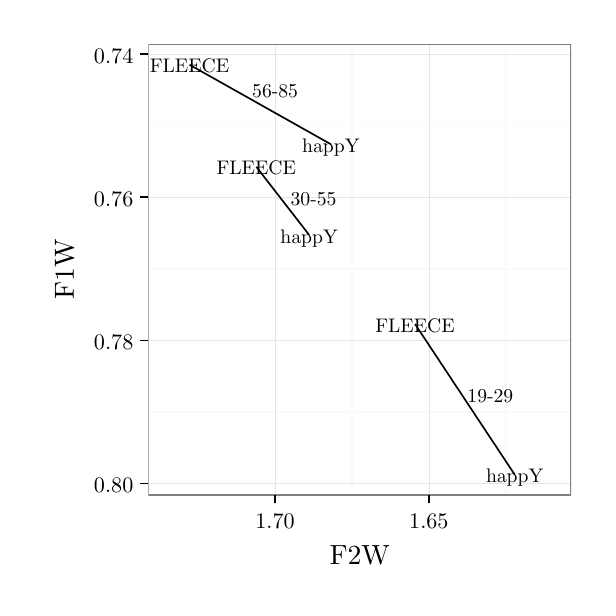
\begin{tikzpicture}[x=1pt,y=1pt]
\definecolor{fillColor}{RGB}{255,255,255}
\path[use as bounding box,fill=fillColor,fill opacity=0.00] (0,0) rectangle (202.36,202.36);
\begin{scope}
\path[clip] (  0.00,  0.00) rectangle (202.36,202.36);
\definecolor{drawColor}{RGB}{255,255,255}
\definecolor{fillColor}{RGB}{255,255,255}

\path[draw=drawColor,line width= 0.6pt,line join=round,line cap=round,fill=fillColor] (  0.00,  0.00) rectangle (202.36,202.36);
\end{scope}
\begin{scope}
\path[clip] ( 43.58, 33.48) rectangle (196.36,196.36);
\definecolor{fillColor}{RGB}{255,255,255}

\path[fill=fillColor] ( 43.58, 33.48) rectangle (196.36,196.36);
\definecolor{drawColor}{gray}{0.98}

\path[draw=drawColor,line width= 0.6pt,line join=round] ( 43.58,166.97) --
	(196.36,166.97);

\path[draw=drawColor,line width= 0.6pt,line join=round] ( 43.58,115.23) --
	(196.36,115.23);

\path[draw=drawColor,line width= 0.6pt,line join=round] ( 43.58, 63.50) --
	(196.36, 63.50);

\path[draw=drawColor,line width= 0.6pt,line join=round] (172.74, 33.48) --
	(172.74,196.36);

\path[draw=drawColor,line width= 0.6pt,line join=round] (117.19, 33.48) --
	(117.19,196.36);
\definecolor{drawColor}{gray}{0.90}

\path[draw=drawColor,line width= 0.2pt,line join=round] ( 43.58,192.83) --
	(196.36,192.83);

\path[draw=drawColor,line width= 0.2pt,line join=round] ( 43.58,141.10) --
	(196.36,141.10);

\path[draw=drawColor,line width= 0.2pt,line join=round] ( 43.58, 89.36) --
	(196.36, 89.36);

\path[draw=drawColor,line width= 0.2pt,line join=round] ( 43.58, 37.63) --
	(196.36, 37.63);

\path[draw=drawColor,line width= 0.2pt,line join=round] (144.97, 33.48) --
	(144.97,196.36);

\path[draw=drawColor,line width= 0.2pt,line join=round] ( 89.41, 33.48) --
	( 89.41,196.36);
\definecolor{drawColor}{RGB}{0,0,0}

\node[text=drawColor,anchor=base,inner sep=0pt, outer sep=0pt, scale=  0.71] at (109.55,157.29) {happY};

\node[text=drawColor,anchor=base,inner sep=0pt, outer sep=0pt, scale=  0.71] at ( 58.51,186.01) {FLEECE};

\node[text=drawColor,anchor=base,inner sep=0pt, outer sep=0pt, scale=  0.71] at (101.71,124.53) {happY};

\node[text=drawColor,anchor=base,inner sep=0pt, outer sep=0pt, scale=  0.71] at ( 82.62,149.14) {FLEECE};

\node[text=drawColor,anchor=base,inner sep=0pt, outer sep=0pt, scale=  0.71] at (175.97, 37.94) {happY};

\node[text=drawColor,anchor=base,inner sep=0pt, outer sep=0pt, scale=  0.71] at (139.97, 92.33) {FLEECE};

\path[draw=drawColor,line width= 0.6pt,line join=round] (109.55,160.23) --
	( 58.51,188.95);

\path[draw=drawColor,line width= 0.6pt,line join=round] (101.71,127.47) --
	( 82.62,152.08);

\path[draw=drawColor,line width= 0.6pt,line join=round] (175.97, 40.88) --
	(139.97, 95.27);

\node[text=drawColor,anchor=base,inner sep=0pt, outer sep=0pt, scale=  0.71] at ( 89.41,176.96) {56-85};

\node[text=drawColor,anchor=base,inner sep=0pt, outer sep=0pt, scale=  0.71] at (103.30,138.16) {30-55};

\node[text=drawColor,anchor=base,inner sep=0pt, outer sep=0pt, scale=  0.71] at (167.19, 67.02) {19-29};
\definecolor{drawColor}{gray}{0.50}

\path[draw=drawColor,line width= 0.6pt,line join=round,line cap=round] ( 43.58, 33.48) rectangle (196.36,196.36);
\end{scope}
\begin{scope}
\path[clip] (  0.00,  0.00) rectangle (202.36,202.36);
\definecolor{drawColor}{RGB}{0,0,0}

\node[text=drawColor,anchor=base east,inner sep=0pt, outer sep=0pt, scale=  0.80] at ( 38.18,189.53) {0.74};

\node[text=drawColor,anchor=base east,inner sep=0pt, outer sep=0pt, scale=  0.80] at ( 38.18,137.79) {0.76};

\node[text=drawColor,anchor=base east,inner sep=0pt, outer sep=0pt, scale=  0.80] at ( 38.18, 86.06) {0.78};

\node[text=drawColor,anchor=base east,inner sep=0pt, outer sep=0pt, scale=  0.80] at ( 38.18, 34.32) {0.80};
\end{scope}
\begin{scope}
\path[clip] (  0.00,  0.00) rectangle (202.36,202.36);
\definecolor{drawColor}{RGB}{0,0,0}

\path[draw=drawColor,line width= 0.6pt,line join=round] ( 40.58,192.83) --
	( 43.58,192.83);

\path[draw=drawColor,line width= 0.6pt,line join=round] ( 40.58,141.10) --
	( 43.58,141.10);

\path[draw=drawColor,line width= 0.6pt,line join=round] ( 40.58, 89.36) --
	( 43.58, 89.36);

\path[draw=drawColor,line width= 0.6pt,line join=round] ( 40.58, 37.63) --
	( 43.58, 37.63);
\end{scope}
\begin{scope}
\path[clip] (  0.00,  0.00) rectangle (202.36,202.36);
\definecolor{drawColor}{RGB}{0,0,0}

\path[draw=drawColor,line width= 0.6pt,line join=round] (144.97, 30.48) --
	(144.97, 33.48);

\path[draw=drawColor,line width= 0.6pt,line join=round] ( 89.41, 30.48) --
	( 89.41, 33.48);
\end{scope}
\begin{scope}
\path[clip] (  0.00,  0.00) rectangle (202.36,202.36);
\definecolor{drawColor}{RGB}{0,0,0}

\node[text=drawColor,anchor=base,inner sep=0pt, outer sep=0pt, scale=  0.80] at (144.97, 21.47) {1.65};

\node[text=drawColor,anchor=base,inner sep=0pt, outer sep=0pt, scale=  0.80] at ( 89.41, 21.47) {1.70};
\end{scope}
\begin{scope}
\path[clip] (  0.00,  0.00) rectangle (202.36,202.36);
\definecolor{drawColor}{RGB}{0,0,0}

\node[text=drawColor,anchor=base,inner sep=0pt, outer sep=0pt, scale=  1.00] at (119.97,  8.40) {F2W};
\end{scope}
\begin{scope}
\path[clip] (  0.00,  0.00) rectangle (202.36,202.36);
\definecolor{drawColor}{RGB}{0,0,0}

\node[text=drawColor,rotate= 90.00,anchor=base,inner sep=0pt, outer sep=0pt, scale=  1.00] at ( 16.67,114.92) {F1W};
\end{scope}
\end{tikzpicture}
